\documentclass[10pt,journal]{IEEEtran}
\usepackage{amsmath,amssymb,booktabs,graphicx,cite}
\usepackage{tikz}
\usetikzlibrary{arrows.meta,positioning,fit}
\usepackage{flushend}
\usepackage[hidelinks]{hyperref}
\newtheorem{theorem}{Theorem}
\newtheorem{proposition}{Proposition}
\newtheorem{lemma}{Lemma}
\newtheorem{corollary}{Corollary}
\newtheorem{remark}{Remark}
\newcommand{\E}{\mathbb E}
\newcommand{\M}{\mathcal M}
\newcommand{\Sset}{\mathcal S}
\newcommand{\KL}{D_{\mathrm{KL}}}
\newcommand{\KLb}{D_{\mathrm{KL},2}}
\newcommand{\snr}{\mathsf{SNR}}
\DeclareMathOperator{\diag}{diag}
\DeclareMathOperator{\tr}{tr}
\DeclareMathOperator{\conv}{conv}
\DeclareMathOperator{\dist}{dist}
\DeclareMathOperator{\rank}{rank}
\title{Semantic Rate--Distortion on a Task Manifold: Object Versus Predictive Receivers and Their Channel Limits}
\author{} % Insert the confirmed author list and affiliations before submission.
\begin{document}
\maketitle
\begin{abstract}
The rate needed for a given task fidelity depends on what a semantic receiver is allowed to output. We study a conditional semantic source on a task manifold and compare an object receiver, which must return a realizable representation, with a predictive receiver, which may return any distribution over task outcomes. An exact identity splits the end-to-end log loss into Bayes, representation, compression, channel and decoder terms. The predictive rate--distortion function is an information bottleneck curve. The object receiver adds a projection term that vanishes for every source if and only if the set of realizable posteriors is convex. We bound this price from below and above, and show that locally it equals half the squared mixture curvature times the squared distortion. At high resolution both receivers obey a task-rank law whose slope is set by the rank $r$ of the Fisher pullback, which gives the distortion--SNR exponent $2\kappa/r$ over a Gaussian channel with $\kappa$ uses per observation. At a KL distortion of 0.10 bit a 24-state object receiver needs at least 0.6723 bit per observation, whereas a predictive grid achieves 0.4137 bit. On 2,048 held-out CIFAR-100 representations, posterior-KL selection raises eight-bit coarse-label accuracy from 43.31\% to 68.90\%.
\end{abstract}
\begin{IEEEkeywords}
Rate--distortion theory, semantic communication, indirect source coding, information geometry, information bottleneck, joint source--channel coding.
\end{IEEEkeywords}

\section{Introduction}
\IEEEPARstart{W}{hen} a receiver predicts a class from a compressed feature, it may report an average of several plausible posteriors. A receiver that must return an actual object, such as a latent vector for a generative decoder or an entry of a shared knowledge base, may have no object whose posterior equals that average. The difficulty persists with perfect calibration, a noiseless bit pipe and an encoder designed for the task. It comes from the geometry of the admissible outputs. A second difficulty appears over a physical link. A mutual-information optimum is a source-coding benchmark, while a packet format, a fading state and a detector determine which operating points a receiver attains. A theory that guides semantic communication design has to keep these effects apart and assign to each a cost in rate or in channel resources.

\subsection{Related Work}
\emph{Semantic and goal-oriented rate--distortion.} Indirect source coding places the fidelity criterion on a variable observed through the source \cite{dobrushin1962information,wolf1970transmission,witsenhausen1980indirect}, and \cite{liu2022indirect} develops this view for semantic sources. Goal-oriented formulations add fidelity constraints on the observation \cite{Stavrou_2023}, side information \cite{Guo_2026}, task-specific distortions \cite{Chai_2025} and posterior design under computational limits \cite{akyol2026semanticratedistortionposterior}. Synonymous-mapping theories modify the entropy and rate--distortion functionals themselves \cite{niu2024mathematical,zhao2025semanticrd}. Under logarithmic loss the reproduction is a distribution \cite{courtade2014multiterminal,yadav2026loglikelihoodlosssemanticcompression}, and the resulting problem is the information bottleneck \cite{tishby1999information,harremoes2007information,armstrong2026sourcesidesufficiencyinformationbottleneck}, which also underlies learned task-oriented transceivers \cite{shao2022taskoriented,xie2021deepsc,bourtsoulatze2019deep,gunduz2023beyond}. Numerical tools include extended Blahut--Arimoto iterations \cite{Han_2025} and neural estimators \cite{li2024fundamental,yang_sandwich}. These works fix one reproduction alphabet. They do not quantify what changes when the output must be a realizable object.

\emph{Geometry of learned representations.} Pulling a distributional metric back through a decoder gives a Riemannian geometry on a latent space \cite{arvanitidis2021latentspaceodditycurvature,arvanitidis2022pullinginformationgeometry}, and softmax heads induce a dually flat structure used for probing \cite{park2026informationgeometrysoftmaxprobing}. Data-driven metrics and intrinsic dimension can be estimated from denoisers \cite{bamberger2026metric,pmlr-v235-stanczuk24a}, Fisher geometry has been used to describe language-model latents and compression objectives \cite{mabrok2026latent,wang2026geoibgeometryawareinformationbottleneck}, and large collections of frozen representations are now public \cite{pandolfo2026semasialargescaledatasetsemantically}. The manifold hypothesis itself can fail on real embeddings \cite{Robinson_2025}. This literature supplies metrics and dimensions. It does not convert them into rate.

\emph{Rate--distortion on singular and curved sources.} High-resolution theory covers locally quadratic distortions \cite{linder1999high}, sources supported on rectifiable sets \cite{koliander2016entropy}, general metric spaces \cite{riegler2023lossy} and quantization on Riemannian manifolds \cite{iacobelli2016quantization}. Bregman clustering identifies the conditional mean as the optimal unconstrained representative \cite{JMLR:v6:banerjee05b}, and Bregman divergences restricted to curved parameter sets have been studied recently \cite{nielsen2026curvedrepresentationalbregmandivergences}. The gap between a curved reproduction set and its convex hull has not been related to an information budget.

\subsection{Contributions}
We fix the task, the shared context, the cost and the output alphabet before any channel is optimized, and obtain the following results.
\begin{itemize}
\item \emph{System model and loss budget.} A model with shared knowledge, a frozen reference representation, three receiver types and a fading link (Section~\ref{sec:model}). Theorem~\ref{thm:budget} decomposes the receiver log loss exactly into Bayes, representation, compression, channel and decoder terms. The predictive receiver then has an information bottleneck rate--distortion function, and the object receiver pays an additional directed projection.
\item \emph{Price of an object.} The two receivers coincide for every source if and only if the realizable posterior set is convex (Proposition~\ref{prop:convex}). Theorem~\ref{thm:gap} bounds the gap from below when both encoders are optimized independently at the same information, Theorem~\ref{thm:reach} bounds it from above through the reach, and Proposition~\ref{prop:local} identifies its local constant as half the squared mixture curvature.
\item \emph{High-resolution laws.} For task-faithful KL distortion both receivers satisfy $R(D)=h_F-\tfrac r2\ln(4\pi eD/r)+o(1)$ with $r$ the rank of the Fisher pullback (Theorem~\ref{thm:rank}). Corollaries quantify a change of metric, shared knowledge and context-dependent dimension.
\item \emph{Channel limits.} A converse with ergodic and outage forms, the distortion--SNR exponent $2\kappa/r$, and a closed-form analog allocation that assigns more power to weak modes, the opposite of water-filling (Section~\ref{sec:channel}).
\item \emph{Certificates and evidence.} Dual brackets for a declared finite alphabet with a sensitivity bound (Section~\ref{sec:ba}), a posterior-circle study that reproduces every constant above, and paired measurements on frozen image representations (Section~\ref{sec:results}).
\end{itemize}

\emph{Notation.} $I_2,H_2,h_2$ use logarithms to base two and $I,H$ natural logarithms. $\KL$ is in nats and $\KLb=\KL/\ln2$. $\Delta$ is the probability simplex on the task alphabet $\mathcal Y$, and its affine hull with the Euclidean norm $\|\cdot\|$ is the mixture plane. $[x]_+=\max\{x,0\}$.

\begin{figure*}[t]\centering
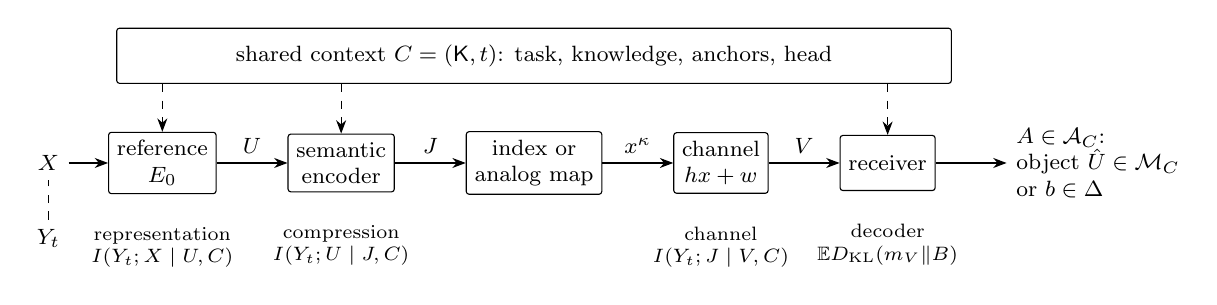
\begin{tikzpicture}[font=\footnotesize,>={Stealth[length=1.7mm]},
 box/.style={draw,rounded corners=1pt,minimum height=7mm,inner sep=3pt,align=center},node distance=7mm]
\node (x) {$X$};
\node[box,right=5mm of x] (e0) {reference\\$E_0$};
\node[box,right=9mm of e0] (enc) {semantic\\encoder};
\node[box,right=9mm of enc] (map) {index or\\analog map};
\node[box,right=9mm of map] (ch) {channel\\$hx+w$};
\node[box,right=9mm of ch] (dec) {receiver};
\node[right=9mm of dec,align=left] (a) {$A\in\mathcal A_C$:\\object $\hat U\in\M_C$\\or $b\in\Delta$};
\node[below=5mm of x] (y) {$Y_t$};
\node[box,above=6mm of map,minimum width=106mm] (ctx) {shared context $C=(\mathsf K,t)$: task, knowledge, anchors, head};
\draw[->] (x)--(e0);
\draw[->] (e0)--node[above]{$U$}(enc);
\draw[->] (enc)--node[above]{$J$}(map);
\draw[->] (map)--node[above]{$x^{\kappa}$}(ch);
\draw[->] (ch)--node[above]{$V$}(dec);
\draw[->] (dec)--(a);
\draw[dashed] (y)--(x);
\draw[dashed,->] (e0.north |- ctx.south)--(e0.north);
\draw[dashed,->] (enc.north |- ctx.south)--(enc.north);
\draw[dashed,->] (dec.north |- ctx.south)--(dec.north);
\node[below=3mm of enc,align=center,font=\scriptsize] (l1) {compression\\$I(Y_t;U\mid J,C)$};
\node[below=3mm of e0,align=center,font=\scriptsize] (l0) {representation\\$I(Y_t;X\mid U,C)$};
\node[below=3mm of ch,align=center,font=\scriptsize] (l2) {channel\\$I(Y_t;J\mid V,C)$};
\node[below=3mm of dec,align=center,font=\scriptsize] (l3) {decoder\\$\E\KL(m_V\Vert B)$};
\end{tikzpicture}
\caption{System model. A frozen reference encoder maps the observation to a representation on the task manifold. The semantic encoder produces a message that crosses a fading link with $\kappa$ uses per observation. The receiver returns an admissible action. The terms below the blocks are the four reducible parts of the log loss in Theorem~\ref{thm:budget}.}
\label{fig:system}\end{figure*}

\section{System Model}\label{sec:model}
\subsection{Semantic Source, Shared Knowledge and Task}
Fig.~\ref{fig:system} shows the model. A sensor produces an observation $X$. The task is to act on a variable $Y_t$ with finite alphabet $\mathcal Y$, such as a class label, that is never observed. The context $C=(\mathsf K,t)$ collects the task index and the knowledge that both terminals hold before transmission: reference models, anchor dictionaries and prediction heads. A sample label is not part of the context. A fixed reference encoder gives the representation
\begin{equation}
 U=E_0(X,C)\in\M_c\subset\mathbb R^d ,\qquad U\mid\{C=c\}\sim\mu_c .
\end{equation}
The tuples $(X,Y_t,C)$ are independent and identically distributed over time. The task posterior of a representation is
\begin{equation}
 Q=q(U,C),\qquad q(u,c)=P(Y_t=\cdot\mid U=u,C=c)\in\Delta ,
\end{equation}
and $\Sset_c=q(\M_c,c)$ is the set of \emph{realizable posteriors}. The geometric results assume that $\M_c$ is a compact smooth embedded manifold of dimension $m_c\ll d$. This is a hypothesis about a learned representation that can be tested and can fail \cite{Robinson_2025}. The finite certificates of Section~\ref{sec:ba} do not need it.

\subsection{Three Receivers}
The receiver returns an action $A\in\mathcal A_c$ and is charged a cost $\delta_c(u,a)$. Three choices of $(\mathcal A_c,\delta_c)$ define three different problems.
\begin{itemize}
\item \emph{Object reconstruction.} $\mathcal A_c=\M_c$ and $\delta_c(u,\hat u)=d_{g_c}(u,\hat u)^2$ for a fixed Riemannian metric $g_c$. The cost measures displacement along the semantic geometry.
\item \emph{Task-faithful object reconstruction (object receiver).} $\mathcal A_c=\M_c$ and $\delta_c(u,\hat u)=\KL(q(u,c)\Vert q(\hat u,c))$. Equivalently the receiver predicts with a realizable posterior $b\in\Sset_c$.
\item \emph{Predictive reproduction (predictive receiver).} $\mathcal A_c=\Delta$ and $\delta_c(u,b)=\KL(q(u,c)\Vert b)$.
\end{itemize}
The last two share the directed loss and differ only in the action set. With the true posterior, $\KLb(Q\Vert b)$ is the excess expected log loss of predicting $b$ from $U$. A frozen classifier head in an experiment defines a proxy criterion whose relation to the label must be measured separately. A point-to-support distance is not among the costs. It vanishes for any two states of the same support and cannot score a confusion between them.

\subsection{Local Task Geometry}
If the entries of $q$ are positive and twice differentiable in a chart, Taylor expansion and $\sum_iq_i=1$ give
\begin{align}
 \KL(q(u)\Vert q(u+v))&=\tfrac12 v^\top G_q(u)v+o(\|v\|^2),\label{eq:fisher}\\
 G_q(u)&=J_q(u)^\top\diag(1/q_i(u))J_q(u),\nonumber
\end{align}
the pullback of the Fisher--Rao metric through the task head \cite{arvanitidis2022pullinginformationgeometry,amari2000methods}. Its null space contains the directions that are invisible to the task to first order, and its rank $r\le\min\{m,|\mathcal Y|-1\}$ will be called the \emph{task rank}. A quotient manifold requires constant rank. Keeping the semidefinite form, or adding a declared $\eta g_0$ with $\eta>0$, gives two different evaluation models. The local form alone does not identify global geodesics and does not make directed KL symmetric.

\subsection{Link}
The transmitter maps a block of $n$ representations and the context to $\kappa n$ complex symbols with average power at most $P$. The receiver observes
\begin{equation}
 V_\ell=h_\ell x_\ell+w_\ell,\qquad w_\ell\sim\mathcal{CN}(0,N_0), \label{eq:channel}
\end{equation}
knows the gains $h_\ell$, and outputs $n$ actions. Let $\snr=P/N_0$. We consider the Gaussian channel ($h_\ell=1$), ergodic fading with capacity $C_{\rm erg}=\E\log_2(1+|h|^2\snr)$, and quasi-static fading with one gain per codeword. A multi-antenna or multicarrier link with channel knowledge at both ends reduces to parallel modes $h_1,\dots,h_k$ after a singular value decomposition \cite{tse2005fundamentals}. The index codec used in the experiments is a special case. It draws a message $J$ from a finite test channel, sends a fixed-width binary index and looks up an anchor.

\subsection{Rate--Distortion Function and Three Reductions}
For additive expected distortion and context known at both ends, the conditional rate--distortion function (RDF) in bits per observation is
\begin{equation}
 R_\delta(D\mid C)=\inf_{\E\delta_C(U,A)\le D} I_2(U;A\mid C),
 \label{eq:rdf}
\end{equation}
with the usual coding interpretation for long blocks under standard finiteness conditions \cite{berger1971rate,cover2006elements}. A context known to only one terminal needs its own coding model.

\begin{lemma}[Context decomposition]\label{lem:context}
For a discrete context let $R_c$ be the RDF of $(\mu_c,\mathcal A_c,\delta_c)$. Then
\begin{equation}
 R_\delta(D\mid C)=\inf_{\sum_c p_cD_c\le D}\ \sum_c p_cR_c(D_c). \label{eq:context}
\end{equation}
\end{lemma}
\begin{IEEEproof}
Conditioning a feasible kernel on each $c$ gives the lower inequality. Combining kernels within $\epsilon$ of the individual optima gives the reverse.
\end{IEEEproof}
At differentiable interior optima the conditional curves have a common slope. Different contexts may spend different amounts of distortion.

\begin{lemma}[Posterior sufficiency]\label{lem:suff}
If $\delta_c(u,a)$ depends on $u$ only through $q(u,c)$, the RDF of the source $U$ equals the RDF of the source $Q$ with the same actions.
\end{lemma}
\begin{IEEEproof}
Averaging a kernel $P_{A|U}$ over $U$ given $Q$ preserves the law of $(Q,A)$ and costs $I(Q;A)\le I(U;A)$. Conversely $Q$ is a function of $U$.
\end{IEEEproof}
Two reference encoders that induce the same law of $Q$ therefore have the same task RDF, whatever their feature dimensions.

\begin{lemma}[Value of shared knowledge]\label{lem:knowledge}
If $\mathcal A_c$ and $\delta_c$ do not depend on $c$, then
\begin{equation}
 R_\delta(D\mid C)\ \le\ R_\delta(D)\ \le\ R_\delta(D\mid C)+I_2(U;C). \label{eq:gray}
\end{equation}
\end{lemma}
\begin{IEEEproof}
A kernel $P_{A|U}$ that ignores $C$ satisfies $I(U;A\mid C)=I(U;A)-I(A;C)$. For a kernel $P_{A|U,C}$, the induced $P_{A|U}$ has the same distortion and $I(U;A)\le I(U;C)+I(U;A\mid C)$ \cite{gray1973new}.
\end{IEEEproof}
Knowledge that changes the cost, for example by reshaping the metric, is not covered by \eqref{eq:gray}. No general ordering holds in that case, and Corollary~\ref{cor:metric} gives the high-resolution answer.

\section{Where Semantic Fidelity Is Lost}\label{sec:budget}
Let $J$ be the message of the semantic encoder, $V$ the channel output and $B\in\Delta$ the prediction issued by the receiver. Randomized mappings are allowed. The only structural requirement is the chain
\begin{equation}
 Y_t - (X,C) - (U,C) - (J,C) - (V,C) - (B,C), \label{eq:chain}
\end{equation}
in which each variable is conditionally independent of all earlier ones given its predecessor.
\begin{theorem}[Loss budget]\label{thm:budget}
Under \eqref{eq:chain}, with $m_J=\E[Q\mid J,C]$ and $m_V=\E[Q\mid V,C]$,
\begin{align}
 \E[-\log_2B(Y_t)]={}&H_2(Y_t\mid X,C)+I_2(Y_t;X\mid U,C)\nonumber\\
 &+I_2(Y_t;U\mid J,C)+I_2(Y_t;J\mid V,C)\nonumber\\
 &+\E\KLb(m_V\Vert B). \label{eq:budget}
\end{align}
Moreover $I_2(Y_t;U\mid J,C)=\E\KLb(Q\Vert m_J)$ and $I_2(Y_t;J\mid V,C)=\E\KLb(m_J\Vert m_V)$.
\end{theorem}
\begin{IEEEproof}
Given $(V,C)$ the prediction is independent of $Y_t$, so the conditional expected loss is $H_2(P_{Y_t|V,C})+\KLb(P_{Y_t|V,C}\Vert B)$ and $P_{Y_t|V,C}=m_V$ by \eqref{eq:chain}. Hence the left side is $H_2(Y_t\mid V,C)+\E\KLb(m_V\Vert B)$. The chain gives $H(Y_t\mid J,V,C)=H(Y_t\mid J,C)$, $H(Y_t\mid U,J,C)=H(Y_t\mid U,C)$ and $H(Y_t\mid X,U,C)=H(Y_t\mid X,C)$, and telescoping $H(Y_t\mid V,C)$ through these three equalities gives \eqref{eq:budget}. The last two identities write the conditional mutual informations as mean divergences between consecutive conditional laws of $Y_t$.
\end{IEEEproof}
The five terms have distinct owners. The Bayes term belongs to the sensor. The representation term is fixed once $E_0$ is frozen and cannot be removed by any link rate. The compression term is the only one controlled by source coding. The channel term vanishes for a noiseless pipe. The decoder term vanishes exactly when the receiver outputs the posterior mean of what it received. It collects three effects that are often conflated: a realizability constraint ($B$ must lie in $\Sset_c$), a knowledge mismatch (the receiver holds a table $\tilde b_V\ne m_V$), and a decoding rule that ignores channel errors. The reducible loss is a chain of divergences $Q\to m_J\to m_V\to B$ between successive conditional means.

Theorem~\ref{thm:budget} is a chain rule for logarithmic loss \cite{courtade2014multiterminal}. Its use here is to separate what each receiver can optimize. For a noiseless pipe, $V=J$, define in nats
\begin{align}
 D_{\rm pred}(R)&=\min_{I(U;J|C)\le R} I(Y_t;U\mid J,C),\label{eq:dpred}\\
 D_{\rm obj}(R)&=\min_{I(U;J|C)\le R}\big\{I(Y_t;U\mid J,C)\nonumber\\
 &\qquad+\E\min_{b\in\Sset_C}\KL(m_J\Vert b)\big\}.\label{eq:dobj}
\end{align}
The first is the information bottleneck tradeoff $I(Y_t;U\mid C)-\max I(Y_t;J\mid C)$ \cite{tishby1999information,harremoes2007information}. By Lemma~\ref{lem:suff} both are functions of the law of $Q$ only, and they are the distortion--rate functions of the predictive and object receivers of Section~\ref{sec:model}.

\section{The Price of an Object}\label{sec:gap}
Fix a context and write $\Sset=q(\M)$. Throughout this section $\Sset$ is compact and every coordinate of every $s\in\Sset$ is at least $\eta>0$. For an encoder with message $J$ let
\begin{equation}
 d_J=\E[\KL(Q\Vert m_J)\mid J],\qquad v_J=\E[\|Q-m_J\|^2\mid J].
\end{equation}
\begin{proposition}[Centroid and projection]\label{prop:centroid}
For each admissible prediction $b_J$ with finite expected loss,
\begin{equation}
 \E\KL(Q\Vert b_J)=\E\KL(Q\Vert m_J)+\E\KL(m_J\Vert b_J). \label{eq:centroid}
\end{equation}
With unrestricted actions the second term can be zero. With an object receiver its infimum for the fixed encoder is the mean directed projection cost of $m_J$ onto $\Sset$.
\end{proposition}
\begin{IEEEproof}
This is the noiseless case of Theorem~\ref{thm:budget}, and the Bregman centroid identity of \cite{JMLR:v6:banerjee05b}. On a compact set of strictly positive posteriors the pointwise minimum is attained and admits a measurable selection.
\end{IEEEproof}
The projection $\min_{b\in\Sset}\KL(m\Vert b)$ is the $m$-projection of information geometry \cite{amari2000methods}. It is unique when $\Sset$ is an exponential family, as for a softmax head on an affine feature set, yet its value is positive unless $m\in\Sset$.

\begin{proposition}[Convexity characterization]\label{prop:convex}
$D_{\rm obj}(R)=D_{\rm pred}(R)$ for every source law on $\Sset$ and every $R\ge0$ if and only if $\Sset$ is convex.
\end{proposition}
\begin{IEEEproof}
If $\Sset$ is convex and closed, every conditional mean $m_J$ lies in $\Sset$ and the projection term in \eqref{eq:dobj} vanishes. Otherwise there are $a,b\in\Sset$ and $\lambda\in(0,1)$ with $m=\lambda a+(1-\lambda)b\notin\Sset$. For the two-point source on $\{a,b\}$ with weights $(\lambda,1-\lambda)$, a zero-rate receiver outputs a constant, because an independently randomized action cannot beat the best constant. The predictive optimum is $m$, and the object receiver pays in addition $\min_{s\in\Sset}\KL(m\Vert s)>0$ by compactness.
\end{IEEEproof}
Thus the price is a property of the mixture geometry of $\Sset$. A posterior family that is flat in the exponential sense but not in the mixture sense has a positive price for some source. At zero rate the exact excess is $\min_{b\in\Sset}\KL(\E Q\Vert b)$. For positive rate an object encoder might change its partition to avoid expensive projections. The next bound allows that reoptimization.

\begin{theorem}[Separation at equal information]\label{thm:gap}
Suppose $\Sset\subset\{q:\varphi(q)=0\}$ for a function $\varphi$ that is $\kappa_\varphi$-strongly convex and $L$-Lipschitz on $\conv(\Sset)$ with respect to the Euclidean norm of the mixture plane. Then, for every source law on $\Sset$ and every $R\ge0$, in nats,
\begin{equation}
 D_{\rm obj}(R)\ \ge\ D_{\rm pred}(R)+\gamma\,D_{\rm pred}(R)^2,\quad
 \gamma=\Big(\frac{\kappa_\varphi\eta}{2L}\Big)^2 . \label{eq:gap}
\end{equation}
\end{theorem}
\begin{IEEEproof}
Consider any feasible object encoder and take its output as the message $J$. Given $J$ write $m,v,d$ for $m_J,v_J,d_J$. The function $\varphi(q)-\kappa_\varphi\|q\|^2/2$ is convex, so Jensen's inequality yields $\varphi(m)\le\E[\varphi(Q)\mid J]-\kappa_\varphi v/2=-\kappa_\varphi v/2$. For any $b\in\Sset$, Lipschitz continuity gives $\|b-m\|\ge\kappa_\varphi v/(2L)$. A zero-sum vector satisfies $\|z\|_1^2\ge2\|z\|_2^2$ by splitting its positive and negative parts, so Pinsker's inequality gives $\KL(m\Vert b)\ge\|m-b\|^2\ge\kappa_\varphi^2v^2/(4L^2)$. Also $\ln t\le t-1$ and $m_i\ge\eta$ give $d\le v/\eta$. Substitution into \eqref{eq:centroid} and Jensen's inequality bound the object loss below by $\E d+\gamma(\E d)^2$. The free decoder $m_J$ is feasible for the predictive receiver at the same information, hence $\E d\ge D_{\rm pred}(R)$, and $x\mapsto x+\gamma x^2$ is increasing. Taking the infimum over object encoders proves \eqref{eq:gap}.
\end{IEEEproof}
For distortion in bits the coefficient is multiplied by $\ln2$. The inequality is strict whenever $D_{\rm pred}(R)>0$. Ellipsoidal level sets inside the simplex satisfy the assumptions, with $\kappa_\varphi$ the least eigenvalue of the quadratic form on the mixture plane. For discrete contexts with coefficients $\gamma_c>0$ the same proof and the Cauchy--Schwarz inequality $\E[\gamma_Cd_C^2]\ge(\E d_C)^2/\E[\gamma_C^{-1}]$ give the harmonic coefficient $(\E\gamma_C^{-1})^{-1}$.

\begin{corollary}[Posterior circle]\label{cor:circle}
Let $q_i(\theta)=1/3+a\cos(\theta-2\pi i/3)$, $i=0,1,2$, with $0<a<1/3$, and put $c=(1,1,1)/3$, $r_\circ=\sqrt{3/2}\,a$, $\eta=1/3-a$. Then \eqref{eq:gap} holds with $\gamma=\eta^2/(4r_\circ^2)$. For uniform $\theta$ the zero-rate price in bits is exactly
\begin{equation}
 -\tfrac13\log_2\!\big[1-27a^2(1-a)/4\big]. \label{eq:zero}
\end{equation}
\end{corollary}
\begin{IEEEproof}
Take $\varphi(q)=(\|q-c\|^2-r_\circ^2)/2$, for which $\kappa_\varphi=1$ and $L=r_\circ$ on the disk. For uniform $\theta$, $\E Q=c$ and $\KLb(c\Vert q)=-\frac13\log_2(27\prod_iq_i)$. The three-phase cosines have zero sum, pairwise products summing to $-3/4$ and triple product $\cos(3\theta)/4$, so $27\prod_iq_i=1-27a^2/4+27a^3\cos(3\theta)/4$, which is maximal at $\theta=0$.
\end{IEEEproof}
At $a=0.2$ the price is 0.117025 bit, and the predictive and object zero-rate losses are 0.136536 and 0.253561 bit (Fig.~\ref{fig:posterior}).

\begin{corollary}[Rate form]\label{cor:rate}
Let $R_{\rm obj},R_{\rm pred}$ be the inverse functions of $D_{\rm obj},D_{\rm pred}$ and $\psi(D)=(\sqrt{1+4\gamma D}-1)/(2\gamma)<D$. Under the assumptions of Theorem~\ref{thm:gap},
\begin{equation}
 R_{\rm obj}(D)\ \ge\ R_{\rm pred}(\psi(D))\ \ge\ R_{\rm pred}(D)+\beta_D\,(D-\psi(D)),
\end{equation}
where $-\beta_D$ is any subgradient of the convex function $R_{\rm pred}$ at $D$, and $D-\psi(D)=\gamma D^2+O(D^3)$.
\end{corollary}
\begin{IEEEproof}
If $D_{\rm obj}(R)\le D$ then $D_{\rm pred}(R)\le\psi(D)$ by \eqref{eq:gap}, so $R\ge R_{\rm pred}(\psi(D))$. The second inequality is the supporting line.
\end{IEEEproof}

\begin{figure*}[t]\centering
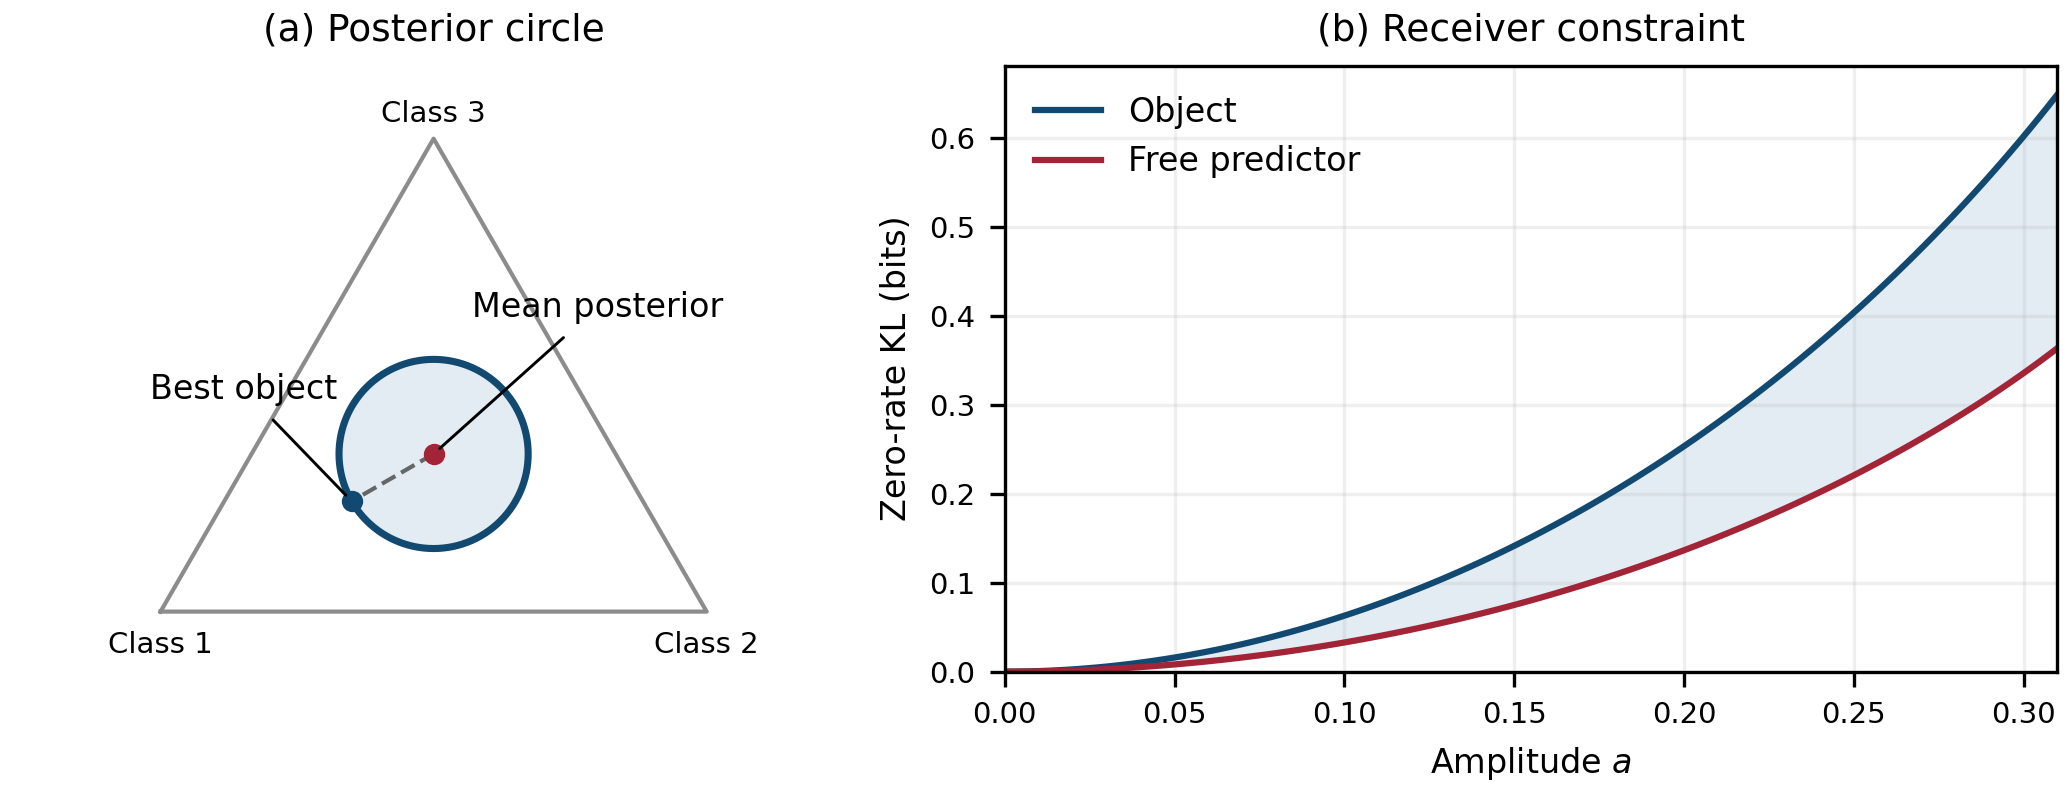
\includegraphics[width=.8\textwidth]{figures/toy_posterior_manifold.png}
\caption{On the posterior circle the mean of a uniform source lies inside the disk. Predicting that mean attains the free zero-rate optimum. Requiring an object moves the prediction to the circle and incurs the shaded excess KL of \eqref{eq:zero}.}
\label{fig:posterior}\end{figure*}

\subsection{An Upper Bound Through the Reach}
The reach of a closed set is the largest $\tau$ such that every point at distance less than $\tau$ has a unique nearest point in the set \cite{federer1959curvature}. A compact $C^2$ submanifold has positive reach.
\begin{lemma}[Centroid defect]\label{lem:defect}
Let $\Sset\subset\mathbb R^N$ be closed with reach $\tau>0$, and let $Q$ be an $\Sset$-valued random vector with mean $m$ and variance $v=\E\|Q-m\|^2<\tau^2$. Then
\begin{equation}
 \dist(m,\Sset)\ \le\ \tau-\sqrt{\tau^2-v}\ \le\ v/\tau .
\end{equation}
\end{lemma}
\begin{IEEEproof}
Let $a$ be a nearest point of $\Sset$ to $m$ and $\rho=\|m-a\|$. Since $\rho\le\|m-Q\|$ for every realization, $\rho^2\le v<\tau^2$. If $\rho>0$ let $n=(m-a)/\rho$. For $t<\tau$ the point $a+tn$ has $a$ as its unique nearest point \cite[Th.~4.8]{federer1959curvature}, so the open ball of radius $t$ about it contains no point of $\Sset$. Hence $\|Q-a-tn\|^2\ge t^2$, that is $\langle Q-a,n\rangle\le\|Q-a\|^2/(2t)$, and letting $t\uparrow\tau$ and taking expectations gives $\rho\le(v+\rho^2)/(2\tau)$. The quadratic inequality and $\rho<\tau$ leave only $\rho\le\tau-\sqrt{\tau^2-v}$.
\end{IEEEproof}
\begin{theorem}[Rounding to an object]\label{thm:reach}
Let $\Sset$ have reach $\tau$ in the mixture plane. For any encoder with $d_J<\tau^2$ almost surely, the receiver that outputs a nearest point of $\Sset$ to $m_J$ attains, at the same information,
\begin{equation}
 D_{\rm obj}\ \le\ \E d_J+\frac{\E[d_J^2]}{\eta\,\tau^2}. \label{eq:round}
\end{equation}
\end{theorem}
\begin{IEEEproof}
Pinsker's inequality and $\|z\|_2^2\le\|z\|_1^2/2$ give $v_J\le d_J$. By Lemma~\ref{lem:defect} there is $b_J\in\Sset$ with $\|m_J-b_J\|\le v_J/\tau$, measurable in $m_J$ because the nearest-point map is continuous inside the reach. Finally $\KL(m\Vert b)\le\sum_i(m_i-b_i)^2/b_i\le\|m-b\|^2/\eta$.
\end{IEEEproof}
For the circle $\tau=r_\circ$, so the price of any encoder lies between $\gamma(\E d_J)^2$ and $\E[d_J^2]/(\eta r_\circ^2)$. Both are quadratic in the cell distortion. The second moment in \eqref{eq:round} is over messages, and a bound on the mean distortion alone does not control it. For an encoder with $d_J\le\vartheta\,\E d_J$ almost surely, the price is at most $\vartheta(\E d_J)^2/(\eta\tau^2)$.

\subsection{The Local Constant: Mixture Curvature}
The constants in \eqref{eq:gap} and \eqref{eq:round} come from Pinsker-type inequalities and are not sharp. The sharp local constant is geometric. Let $\Sset$ be a $C^3$ embedded submanifold of the open simplex of dimension $r$, with Fisher inner product $\langle z,w\rangle_s=\sum_iz_iw_i/s_i$ on vectors of the mixture plane. For a local parametrization $q(\xi)$ define the \emph{mixture second fundamental form} $\mathrm{I\!I}_{ab}=(\partial_a\partial_bq)^{\perp}$, the Fisher-normal part of the ordinary second derivative. It is the embedding curvature of $\Sset$ for the mixture connection \cite{amari2000methods}, the mixture counterpart of Efron's statistical curvature \cite{efron1975defining}, and it vanishes identically exactly when $\Sset$ is an open piece of a mixture family.
\begin{proposition}[Local price]\label{prop:local}
Let a law on $\Sset$ be supported in a Fisher ball of radius $\epsilon$ about $s\in\Sset$, with mean $m$ and covariance $\Sigma^{ab}$ in coordinates $\xi$ whose metric matrix at $s$ is $G_{ab}$. As $\epsilon\to0$,
\begin{align}
 \E\KL(Q\Vert m)&=\tfrac12G_{ab}\Sigma^{ab}+O(\epsilon^3),\\
 \min_{b\in\Sset}\KL(m\Vert b)&=\tfrac18\big\|\Sigma^{ab}\mathrm{I\!I}_{ab}\big\|_s^2+O(\epsilon^5).
\end{align}
For a curve ($r=1$) with mixture curvature $\kappa_m=\|\mathrm{I\!I}(e,e)\|_s$ along its Fisher-unit tangent $e$, the price of a small cell with distortion $d$ is $\tfrac12\kappa_m^2d^2+O(\epsilon^5)$.
\end{proposition}
\begin{IEEEproof}
Expand about the coordinate mean $\bar\xi$: $m=q(\bar\xi)+\frac12\Sigma^{ab}\partial_a\partial_bq+O(\epsilon^3)$. The first claim follows from \eqref{eq:fisher} and $\|q(\xi)-m\|_s^2=G_{ab}(\xi-\bar\xi)^a(\xi-\bar\xi)^b+O(\epsilon^3)$. For $b=q(\bar\xi+\zeta)$ with $\zeta=O(\epsilon^2)$, $\KL(m\Vert b)=\frac12\|\frac12\Sigma^{ab}\partial_a\partial_bq-\zeta^a\partial_aq\|_s^2+O(\epsilon^5)$, and minimizing over $\zeta$ removes the tangential part. Points $b$ outside a fixed neighborhood cost more than $O(\epsilon^4)$.
\end{IEEEproof}
For an isotropic cell, $\Sigma^{ab}=(2d/r)G^{ab}$ and the price is $d^2\|\mathbf H_m\|_s^2/(2r^2)$ with $\mathbf H_m=G^{ab}\mathrm{I\!I}_{ab}$ the mixture mean curvature vector. Section~\ref{sec:results} shows that on the circle the equal-information gap $D_{\rm obj}(R)-D_{\rm pred}(R)$ divided by $D_{\rm pred}(R)^2$ approaches $\frac12\E\kappa_m^2$ as the rate grows.

\section{High-Resolution Laws on the Task Manifold}\label{sec:highres}
\subsection{Intrinsic Squared Distance}
Suppose $\M$ is compact, smooth and boundaryless of dimension $m$, with a continuous positive density $p$ relative to the volume $dV_g$, on-manifold reproduction and $\delta=d_g^2$. Let $Z_s(a)=\int_\M e^{-s d_g(x,a)^2}dV_g(x)$ and $h_g(p)=-\int p\ln p\,dV_g$. Comparing the conditional law of $U$ given $A=a$ with the Gibbs density about $a$ bounds its conditional entropy by $s\E[d_g^2\mid A=a]+\ln Z_s(a)$. Consequently, for every $s>0$,
\begin{equation}
 R_{\rm nat}(D)\ge h_g(p)-sD-\ln\sup_a Z_s(a). \label{eq:lowergeo}
\end{equation}
In the other direction the kernel $W_s(da\mid u)=e^{-s d_g^2(u,a)}dV_g(a)/Z_s(u)$ has distortion $D_s=-\E\,\partial_s\ln Z_s(U)$ and information
\begin{equation}
 h_g(A_s)-\E\ln Z_s(U)-sD_s. \label{eq:uppergeo}
\end{equation}
Both bounds hold at every finite distortion. Their equality at finite $D$ does not follow from local flatness.
\begin{theorem}[Intrinsic law]\label{thm:intrinsic}
Under the assumptions above, as $D\downarrow0$,
\begin{equation}
 R_{\rm nat}(D)=h_g(p)-\frac m2\ln\frac{2\pi eD}{m}+o(1). \label{eq:highres}
\end{equation}
\end{theorem}
The proof is in Appendix~\ref{app:highres}. Absolute continuity, the metric and the order of limits matter. For a fixed finite empirical cloud the information saturates at its discrete entropy, and fitting the last slopes of such a curve cannot establish \eqref{eq:highres}.

\subsection{Task-Faithful Distortion and the Task Rank}
\begin{theorem}[Task-rank law]\label{thm:rank}
Let $q:\M\to\Delta$ be smooth with positive entries and constant rank $r\ge1$, such that $\Sset=q(\M)$ is a compact embedded $C^3$ submanifold of dimension $r$. Let the law $P_Q$ of $Q$ have a continuous positive density $p_\Sset$ with respect to the Fisher--Rao volume $V_F$ of $\Sset$, and $h_F=-\int p_\Sset\ln p_\Sset\,dV_F$. Then both the object and the predictive receiver satisfy, in nats as $D\downarrow0$,
\begin{equation}
 R(D)=h_F-\frac r2\ln\frac{4\pi eD}{r}+o(1). \label{eq:rank}
\end{equation}
\end{theorem}
The proof is in Appendix~\ref{app:highres}. The density assumption holds when $U$ has a continuous positive density on $\M$, by the coarea formula. Three consequences follow. First, the logarithmic growth is governed by the task rank, which never exceeds $|\mathcal Y|-1$, and neither by the intrinsic dimension $m$ of the representation nor by the feature dimension $d$. Directions in the null space of $G_q$ are free. Second, the constant $h_F$ depends on the reference encoder only through the law of the posterior (Lemma~\ref{lem:suff}). Third, the two receivers share the expansion, so the rate price of an object vanishes at high resolution, in agreement with the quadratic law of Section~\ref{sec:gap}.

\begin{corollary}[Metric, knowledge and dimension]\label{cor:metric}
(i) For two smooth metrics on $\M$, $h_{g'}(p)=h_g(p)+\frac12\E\ln\det(g^{-1}g')$, so $R_{g'}(D)-R_g(D)\to\frac12\E\ln\det(g^{-1}g')$ for squared geodesic costs. (ii) If the context changes only the source law on a common $(\M,g)$, then $R(D)-R(D\mid C)\to I(U;C)$, and the upper bound in \eqref{eq:gray} is asymptotically tight. (iii) If the context selects manifolds of dimensions $m_c$ with entropies $h_c$ on a finite context set, then
\begin{equation}
 R_{\rm nat}(D\mid C)=\sum_cp_ch_c-\frac{\bar m}2\ln\frac{2\pi eD}{\bar m}+o(1),
\end{equation}
with $\bar m=\E m_C$, and the optimal allocation in \eqref{eq:context} is $D_c=Dm_c/\bar m$.
\end{corollary}
\begin{IEEEproof}
(i) The densities relative to the two volumes differ by the factor $\sqrt{\det(g^{-1}g')}$. (ii) Apply \eqref{eq:highres} to each $\mu_c$ and to the mixture, and use $h_g(U)-h_g(U\mid C)=I(U;C)$. (iii) Insert \eqref{eq:highres} in \eqref{eq:context}. All $D_c\le D/p_c$ tend to zero, and stationarity $m_c/(2D_c)=\mathrm{const}$ gives the allocation.
\end{IEEEproof}
Part (i) prices a change of the semantic metric, for example from a knowledge update that reweights task directions, as an expected log-volume ratio. For the regularized pullback $g'=G_q+\eta g_0$ the ratio diverges as $\frac{m-r}{2}\ln\eta$ when $\eta\downarrow0$, which reflects the drop from $m$ to $r$ dimensions in \eqref{eq:rank}. Part (iii) shows that a task which confines the source to lower-dimensional strata is charged the mean dimension.

\section{Channel Limits}\label{sec:channel}
\subsection{Converse, Outage and the SNR Exponent}
\begin{proposition}[Link converse]\label{prop:link}
Consider the link \eqref{eq:channel} with $\kappa$ complex uses per observation. (i) Any scheme over the Gaussian or ergodic fading channel with mean distortion $D$ satisfies $R_\delta(D\mid C)\le\kappa C_{\rm ch}$, with $C_{\rm ch}=\log_2(1+\snr)$ or $C_{\rm erg}$, and every $D$ with $R_\delta(D\mid C)<\kappa C_{\rm ch}$ is achievable with long blocks. (ii) Under quasi-static fading the conditional mean distortion $D(h)$ of any scheme satisfies $R_\delta(D(h)\mid C)\le\kappa\log_2(1+|h|^2\snr)$. Hence, for Rayleigh fading,
\begin{equation}
 \Pr\{D(h)>D\}\ \ge\ 1-\exp\!\Big[-\frac{2^{R_\delta(D|C)/\kappa}-1}{\snr}\Big]. \label{eq:outage}
\end{equation}
(iii) Under the assumptions of Theorem~\ref{thm:rank}, the least distortion attainable over the Gaussian channel obeys, as $\snr\to\infty$,
\begin{equation}
 D^\star(\snr)=\frac{r}{4\pi e}\,e^{2h_F/r}\,(1+\snr)^{-2\kappa/r}\,(1+o(1)). \label{eq:opta}
\end{equation}
\end{proposition}
\begin{IEEEproof}
(i) is the data-processing converse with convexity of the RDF, and source--channel separation \cite{cover2006elements}. (ii) applies the same converse conditionally on the gain, and $|h|^2$ is exponential. (iii) equates \eqref{eq:rank} with $\kappa\ln(1+\snr)$ nats.
\end{IEEEproof}
A deep fade therefore leaves the source RDF unchanged. It lowers the capacity, and the receiver falls back toward the zero-rate loss of Section~\ref{sec:gap}. The exponent $2\kappa/r$ in \eqref{eq:opta} is the number of real channel dimensions per task dimension, a distortion exponent in the sense of \cite{laneman2005source}. For the intrinsic cost of Theorem~\ref{thm:intrinsic} the same argument gives the exponent $2\kappa/m$ and the constant $\frac{m}{2\pi e}e^{2h_g/m}$.

\subsection{One-Shot Analog Mapping and Two Allocation Regimes}
Learned joint source--channel codes send a low-dimensional representation with a few channel uses \cite{bourtsoulatze2019deep}. Their small-noise behavior follows from a local model. Near a point of $\M$ use chart coordinates $z\in\mathbb R^m$, a positive definite task metric $G$ and a cell covariance $\Sigma_z$. In the whitened coordinates $w=G^{1/2}z$ the semantic distortion is $\E\|\hat w-w\|^2$ and $G^{1/2}\Sigma_zG^{1/2}$ has eigenpairs $(\lambda_i,\nu_i)$. The link offers $m$ real modes $y_i=h_ix_i+n_i$ with $n_i\sim\mathcal N(0,\sigma^2)$ and total power $P$. A \emph{mode-aligned} map sends $x_{\pi(i)}=a_i\langle\nu_i,w\rangle$ for a permutation $\pi$, and the receiver forms the unbiased estimate $y_{\pi(i)}/(h_{\pi(i)}a_i)$.
\begin{proposition}[Aligned analog allocation]\label{prop:analog}
Among mode-aligned maps with $\sum_ia_i^2\lambda_i\le P$, the minimum distortion is
\begin{equation}
 D_{\rm an}=\frac{\sigma^2}{P}\Big(\sum_i\frac{\sqrt{\lambda_i}}{h_{\pi(i)}}\Big)^2 ,
\end{equation}
attained when mode $\pi(i)$ receives the power fraction $(\sqrt{\lambda_i}/h_{\pi(i)})/\sum_j(\sqrt{\lambda_j}/h_{\pi(j)})$, and the best pairing orders the $\lambda_i$ and the $h_{\pi(i)}$ in the same sense.
\end{proposition}
\begin{IEEEproof}
The distortion is $\sigma^2\sum_i(h_{\pi(i)}a_i)^{-2}$. The Cauchy--Schwarz inequality gives $(\sum_ia_i^2\lambda_i)(\sum_ih_{\pi(i)}^{-2}a_i^{-2})\ge(\sum_i\sqrt{\lambda_i}/h_{\pi(i)})^2$ with equality for $a_i^2\propto1/(\sqrt{\lambda_i}h_{\pi(i)})$. The rearrangement inequality minimizes $\sum_i\sqrt{\lambda_i}\,h_{\pi(i)}^{-1}$ by pairing large $\lambda_i$ with small $h^{-1}$.
\end{IEEEproof}
The expression is the Cram\'er--Rao form $\tr(G\,G_{\rm obs}^{-1})$ with observation information $G_{\rm obs}=J_f^\top H^\top H J_f/\sigma^2$ for an encoder Jacobian $J_f$, so it also describes smooth nonlinear maps in the small-noise limit. The restriction to aligned maps is natural, since diagonalizing structures are optimal for linear coding over vector Gaussian channels under mean-square criteria \cite{lee1976optimal}. Two regimes must be distinguished. In the analog regime the power on a mode grows as $1/h$: weak modes receive \emph{more} power, because each task direction has to arrive. In the separated regime of Proposition~\ref{prop:link} capacity-achieving water-filling gives weak modes \emph{less} power, and the task directions are protected by the source code through $G$. The analog distortion decays as $P^{-1}$, whereas \eqref{eq:opta} decays as $P^{-2\kappa/r}$. The two exponents agree only at matched bandwidth $2\kappa=r$, where uncoded transmission can be optimal \cite{gastpar2003code}.

\subsection{Finite Packet Interpretation}
The index codec draws a message from a finite test channel and transmits a fixed-width binary index. An $M$-entry dictionary costs $\lceil\log_2M\rceil$ bits per object before channel coding. Uncoded coherent BPSK in AWGN has bit error $\Phi(-\sqrt{2E_b/N_0})$, and a common Rayleigh gain across one index correlates the bit errors. The test-channel information, the fixed payload, the channel uses and the decoded index errors are therefore recorded separately, and Theorem~\ref{thm:budget} assigns the resulting loss to its compression, channel and decoder parts.

\section{Finite Certificates}\label{sec:ba}
Let $p_i$ be the source weights and $c_{ij}$ the costs for a fixed finite receiver alphabet. For a slope $\beta\ge0$, denote by $F(\beta)$ the minimum of $I_2(W)+\beta D(W)$. Given a positive trial mass $\varrho$, compute
\begin{align}
 Z_i&=\sum_j \varrho_j2^{-\beta c_{ij}},&
 W_{ij}&=\varrho_j2^{-\beta c_{ij}}/Z_i,\nonumber\\
 \bar W_j&=\sum_i p_iW_{ij},&
 G_j&=\sum_i p_i2^{-\beta c_{ij}}/Z_i .
\end{align}
Set $U_\beta=I_2(W)+\beta D(W)$ and $L_\beta=-\sum_i p_i\log_2 Z_i-\log_2\max_j G_j$. Then $L_\beta\le F(\beta)\le U_\beta$. To verify the lower bound take $\alpha_i=-\log_2 Z_i-\log_2\max_j G_j$. For each $j$ the weights $p_i2^{\alpha_i-\beta c_{ij}}$ sum to at most one. Applying the relative-entropy inequality to the conditional source given output $j$, then averaging, gives $I_2+\beta D\ge\sum_i p_i\alpha_i$. The upper value follows by using $W$. Updating $\varrho\gets\bar W$ gives the Blahut iteration \cite{blahut1972computation}, and the gap can be checked before convergence.

At a target $D_0$, maximize the lower lines $L_\beta-\beta D_0$ over the computed slopes, and time-share feasible kernels at neighboring distortions for an upper bound. Conversely, at an information budget $R_0$ the lines give the distortion floor $\max_\beta(L_\beta-R_0)/\beta$. With common context, weight the supported values of each conditional problem at the same $\beta$ as in \eqref{eq:context}. This algorithm certifies the declared cost matrix. Shrinking an unknown continuous problem to a sample changes that problem in both its source and its admissible reconstructions.

\subsection{Sensitivity to the Finite Source Weights}
Suppose two input laws $p,\tilde p$ on the same alphabet differ by total variation at most $\epsilon$, and the same $M\ge2$ reconstructions and costs in $[0,c_{\max}]$ are used. Fix $0\le\epsilon\le1-1/M$ and put $u_\epsilon=\epsilon c_{\max}$, $v_\epsilon=h_2(\epsilon)+2\epsilon\log_2 M$. Then, for feasible shifted targets,
\begin{align}
 R_{\tilde p}(D+u_\epsilon)-v_\epsilon&\le R_p(D)\le R_{\tilde p}(D-u_\epsilon)+v_\epsilon . \label{eq:sens}
\end{align}
For any fixed $W$ the distortion changes by at most $u_\epsilon$. The output laws differ by at most $\epsilon$ by contraction of total variation. Coupling them at their total variation distance and bounding either output entropy conditional on the other gives an entropy difference of at most $h_2(\epsilon)+\epsilon\log_2(M-1)$. The conditional row entropy is an expectation of a function in $[0,\log_2 M]$, so it changes by at most $\epsilon\log_2 M$. Combining these bounds for $I=H(A)-H(A\mid U)$ and transferring any feasible kernel proves \eqref{eq:sens}. For the empirical law of $n$ independent samples on $N$ states, $\E\epsilon\le\frac12\sqrt{(N-1)/n}$, which turns \eqref{eq:sens} into a plug-in bracket for the population RDF of the declared alphabets. The statement keeps the anchors and costs fixed. Independently fitting a second head or changing the support violates that premise.

\section{Numerical Evaluation}\label{sec:results}
\subsection{Certified Receiver-Alphabet and Shared-Context Effects}
Take 24 equally spaced posterior-circle source states with $a=0.2$. The object receiver uses the same 24 states. The enlarged alphabet includes the center and four copies of the grid scaled about the center by $1/4,1/2,3/4,1$, giving 97 predictions. For a common context $K\in\{-1,1\}$ with equal probabilities set $p(i\mid K)=(1+0.8K\cos\theta_i)/24$ and keep the object alphabet. The marginal source is still uniform. Table~\ref{tab:finite} reports outward-rounded brackets from 16 supporting slopes. At $D=0.10$ the object lower bound exceeds the enlarged-alphabet upper bound by 0.2587 bit per observation. Shared context separately reduces the rate required of the object receiver by 0.255 bit at both targets. Here $I_2(U;K)=0.25515$ bit, and the Lagrangian saving $F(\beta)-F(\beta\mid K)$ equals 0.24816, 0.25481 and 0.25515 bit at $\beta=8,16,32$. The upper bound in \eqref{eq:gray} is thus met already at moderate distortion, as Corollary~\ref{cor:metric}(ii) predicts in the limit.
\begin{table}[t]
\caption{Certified finite rates in bits per state. The target is forward KL in bits.}\label{tab:finite}\centering
\begin{tabular}{lcc}\toprule
Receiver and context & $D=0.05$ & $D=0.10$\\\midrule
Circle & [1.2595, 1.2601] & [0.6723, 0.6833]\\
Disk grid & [1.1125, 1.1399] & [0.4121, 0.4137]\\
Circle, shared $K$ & [1.0047, 1.0053] & [0.4174, 0.4278]\\\bottomrule
\end{tabular}\end{table}

\subsection{A Complete Loss Budget}
To exercise Theorem~\ref{thm:budget} we enumerate a full link. The observation is uniform on 64 circle states with $a=0.2$, and the reference encoder merges adjacent pairs into 32 representations. The semantic encoder is the Blahut optimum at $\beta=8$ for the object alphabet of the 32 realizable posteriors and has information 0.4707 bit. Its index is sent as five uncoded BPSK bits with bit error $\Phi(-\sqrt{2E_b/N_0})$. Three receivers are compared: a lookup of the object stored under the received index, the $m$-projection of $m_V$ onto the objects, and the unrestricted posterior mean $m_V$. The Bayes and representation terms are 1.44843 and 0.00035 bit in every row of Table~\ref{tab:budget}. The five terms sum to the directly enumerated log loss within $10^{-15}$ bit in all twelve configurations.
\begin{table}[t]
\caption{Reducible terms of the loss budget in bits (32 objects, five-bit index, $\beta=8$). The compression term is 0.09909 in every row.}\label{tab:budget}\centering
\begin{tabular}{lcccc}\toprule
 & & \multicolumn{3}{c}{Decoder term}\\\cmidrule(lr){3-5}
Link & Channel & Lookup & Projection & Mean\\\midrule
Noiseless & 0 & 0.02398 & 0.02398 & 0\\
Gray, 6 dB & 0.00018 & 0.02482 & 0.02413 & 0\\
Natural, 6 dB & 0.00012 & 0.02534 & 0.02418 & 0\\
Gray, 2 dB & 0.00292 & 0.03680 & 0.02670 & 0\\\bottomrule
\end{tabular}\end{table}
Three observations follow. On a noiseless pipe the object constraint alone costs 0.024 bit, a quarter of the compression term. At 2 dB the channel term is only 0.003 bit, yet a lookup receiver loses a further 0.010 bit relative to the projection receiver. Most of the damage of index errors is thus a decoder effect that the receiver can remove without any change at the transmitter. Finally, the bit labeling changes the channel and decoder terms in opposite directions at 6 dB, which a single end-to-end number would hide.

\subsection{Equal-Information Gap and the High-Resolution Laws}
We next approximate the continuous uniform circle by 720 states. The object receiver uses the same 720 points. The predictive receiver is computed by a free-centroid Blahut iteration whose reproduction points move in the simplex, and the object distortion is evaluated at exactly the information of each predictive point by bisection on the slope. These dense-alphabet values are numerical evaluations, not certificates. For this source $h_F=\ln2\pi+\frac12\E\ln g(\theta)=1.02165$ nats, where $g$ is the squared Fisher speed, and the mixture curvature satisfies $\kappa_m^2\in[2.43,18.06]$ with mean 7.607.
\begin{figure*}[t]\centering
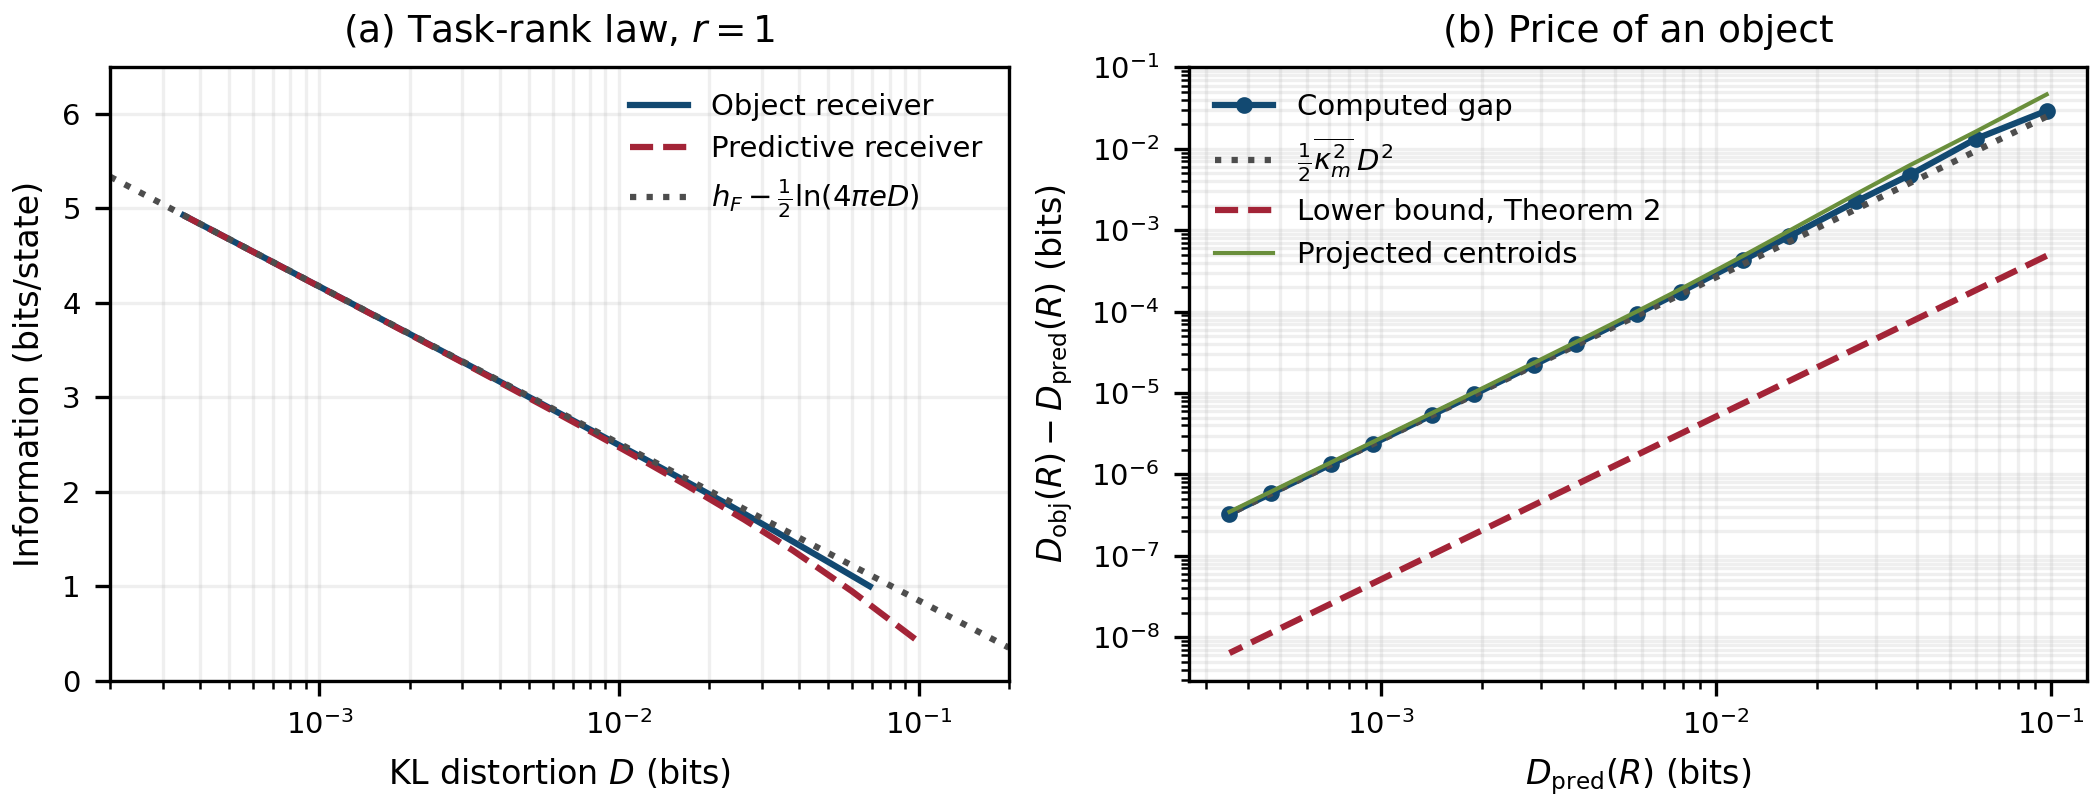
\includegraphics[width=.84\textwidth]{figures/gap_highres.png}
\caption{Posterior circle with 720 states, $a=0.2$. (a) Both receivers approach the task-rank asymptote \eqref{eq:rank} with $r=1$, plotted in bits. (b) The equal-information price of an object follows the local law $\frac12\E[\kappa_m^2]D^2$ of Proposition~\ref{prop:local}. The rigorous lower bound of Theorem~\ref{thm:gap} is valid and about fifty times smaller. Radially projected centroids of the predictive encoder give a constructive upper curve.}
\label{fig:gap}\end{figure*}
\begin{table}[t]
\caption{Equal-information comparison on the 720-state circle. Distortions in bits. The last column is the gap over $D_{\rm pred}^2$ in nats, to be compared with $\frac12\E\kappa_m^2=3.804$.}\label{tab:gap}\centering
\begin{tabular}{rcccc}\toprule
$R$ (bit) & $D_{\rm pred}$ & $D_{\rm obj}-D_{\rm pred}$ & Th.~\ref{thm:gap} bound & Ratio\\\midrule
0.953 & $5.97\!\times\!10^{-2}$ & $1.32\!\times\!10^{-2}$ & $1.83\!\times\!10^{-4}$ & 5.36\\
2.081 & $1.66\!\times\!10^{-2}$ & $8.41\!\times\!10^{-4}$ & $1.41\!\times\!10^{-5}$ & 4.42\\
3.406 & $2.86\!\times\!10^{-3}$ & $2.21\!\times\!10^{-5}$ & $4.20\!\times\!10^{-7}$ & 3.90\\
4.924 & $3.53\!\times\!10^{-4}$ & $3.29\!\times\!10^{-7}$ & $6.39\!\times\!10^{-9}$ & 3.81\\\bottomrule
\end{tabular}\end{table}
Fig.~\ref{fig:gap}(a) and Table~\ref{tab:gap} confirm the three predictions. The asymptote \eqref{eq:rank} exceeds the computed object rate by 0.128, 0.032, 0.005 and 0.0006 bit at the four rates of the table. The price of an object is quadratic in the distortion, and its normalized value decreases to 3.81, within 0.3\% of the mixture-curvature constant. The conditional distortions of the predictive encoder are nearly equal across messages, with $\E d_J^2/(\E d_J)^2\le1.006$, so the rounding bound \eqref{eq:round} applies with $\vartheta\approx1$. Its coefficient $1/(\eta r_\circ^2)=125$ and the coefficient $\gamma=0.074$ of Theorem~\ref{thm:gap} bracket the true constant from far away, which is the cost of their generality. A two-point check of Proposition~\ref{prop:local} at four angles gives ratios within 0.2\% of $\frac12\kappa_m^2$ at half-width 0.05 rad.

\subsection{A Two-Use Gaussian Link}
Transmit $\sqrt{4}(\cos\theta,\sin\theta)$ for the 24-state source over two real Gaussian uses with independent unit-variance noise and known scalar gain $h$. The receiver uses angular maximum-likelihood decisions for $h>0$ and the best constant object at $h=0$. Integrating the two-dimensional normal density over angular decision bins gives Table~\ref{tab:awgn}. The capacity column maximizes over Gaussian inputs under the same energy budget, while the decoded mutual information belongs to this finite constellation. The floor is the certified lower bound of Section~\ref{sec:ba} on the KL of any 24-object scheme whose information does not exceed the capacity, so it holds for every code of any block length (Proposition~\ref{prop:link}).
\begin{table}[t]
\caption{Two real channel uses with total energy four. Information and KL use base-two logarithms.}\label{tab:awgn}\centering
\begin{tabular}{rcccc}\toprule
Gain $h$ & Capacity & Decoded $I_2$ & Task KL & Floor\\\midrule
0 & 0 & 0 & 0.25356 & 0.25356\\
0.5 & 0.5850 & 0.4902 & 0.12823 & 0.10905\\
1 & 1.5850 & 1.3839 & 0.04561 & 0.03316\\
2 & 3.1699 & 2.4941 & 0.01034 & 0.00396\\\bottomrule
\end{tabular}\end{table}
Deep attenuation returns the zero-rate object loss even though the source RDF stays fixed. The one-shot circle map is within 18\% of the floor at $h=0.5$ and a factor 2.6 above it at $h=2$. This widening is the exponent mismatch of Section~\ref{sec:channel}: the map uses two real dimensions for one task dimension and decays as $\snr^{-1}$, while the limit decays as $\snr^{-2}$. As an outage illustration, an object receiver that needs 1.2601 bit per observation ($D=0.05$ in Table~\ref{tab:finite}) over one quasi-static Rayleigh use per observation is in outage with probability at least 13.0\% at 10 dB and 1.39\% at 20 dB by \eqref{eq:outage}.

\subsection{Frozen Representations of Real Images}
SEMASIA provides precomputed representations indexed by backbone, dataset split and image ID \cite{pandolfo2026semasialargescaledatasetsemantically}. We use CIFAR-100 and a 20-way coarse task, for which the task rank is at most 19. The ResNet-18 and MobileNetV3-Small features have dimensions 512 and 1,024. For each backbone a regularized logistic head is fit on 8,192 training images, its temperature is fit on 2,048 other training images, and 2,048 official test IDs are shared across the two measurements. The temperatures are 0.869 and 0.940. Anchors come from training data. The test label evaluates the received decision and is never sent. The experiment uses a noiseless index, so it isolates the choice of task criterion at the sender.
\begin{table}[t]
\caption{Same-backbone reception on 2,048 official test IDs. Accuracy is percent. KL compares the clean and received predictive distributions in bits.}\label{tab:real}\centering
\begin{tabular}{lrrrc}\toprule
Backbone & Payload & Rule & Accuracy & KL\\\midrule
ResNet-18 & 8 & cosine & 43.31 & 2.141\\
          & 8 & KL     & 68.90 & 0.381\\
          & 5 & class  & 72.22 & ---\\
MobileNetV3-S & 8 & cosine & 44.58 & 2.362\\
              & 8 & KL & 70.07 & 0.376\\
              & 5 & class & 72.90 & ---\\\bottomrule
\end{tabular}\end{table}
Both eight-bit rules select among the same 256 IDs. In Table~\ref{tab:real}, KL selection improves decision accuracy by 25.59 and 25.49 percentage points. Sending the most likely class of the head costs five fixed-width bits and preserves its clean classification accuracy. That action returns only a decision, so it has no reconstructed posterior in the table. Under cosine encoding with the posterior of the other backbone at the same received ID, the two directional accuracies are 42.04\% and 41.94\%. Shared sample identity permits this experiment even though the embedding coordinates differ.

A separate $128$-state, $16$-anchor Blahut calculation on each cloud illustrates the distinction between empirical optimization and transmission. At $\beta=2$ the ResNet table attains 2.4291 bits of information at posterior KL 1.9761 bits, with a Lagrangian gap below $10^{-7}$ bit. The MobileNet table gives 1.9337 bits at KL 2.6444 bits with the same gap tolerance. These finite supports and proxy costs differ between backbones. Their rates do not order the population sources.

\section{Discussion}
\emph{What the bounds do and do not say.} Theorem~\ref{thm:gap} is a one-sided inequality for posterior sets with a strongly convex defining function. Saddle-shaped sets admit cells elongated along asymptotic directions whose means stay on the set, and no universal exponent or constant holds for nonconvex supports. Proposition~\ref{prop:local} is a statement about one small cell. Its agreement with the equal-information gap on the circle is numerical evidence, and a proof that the optimal encoders have asymptotically equal cell distortions is open. Theorem~\ref{thm:rank} requires constant rank. A head whose rank drops on a stratum leads to a mixture of dimensions, as in Corollary~\ref{cor:metric}(iii), and to singular strata that need separate control.

\emph{Finite clouds.} A feature cloud supports a discrete study without a manifold identification theorem. For a geometric sensitivity check, the implementation embeds each unit feature $u$ as $(2\sqrt{q(u)},\sqrt{\eta}\,u)$ with frozen $\eta$ and head. Training-only nearest-neighbor edges carry chord lengths. A held-out sample attaches to its training neighbors and takes their shortest training paths to anchors. Squared path lengths and squared chords then give two fixed evaluation matrices. Sampling density, disconnected components and shortcuts must be checked before assigning intrinsic meaning to their difference. Likewise, a change of backbone changes the empirical source, not merely its coordinates.

\emph{From the circle to real data.} The proven separation uses true posteriors and independent optimization of both encoders. The real-image experiment uses a learned head and compares two selection rules on observed anchors. Its accuracy result supports choosing a task-sensitive distortion. Establishing a comparable object--predictor separation on real data requires nested receiver alphabets, matched information and paired uncertainty across independent splits. The fixed-width noisy link additionally changes the payload when the enlarged dictionary requires another bit, and comparing only clean distortion would miss that cost. The loss budget offers a protocol for such a study: report the five terms of \eqref{eq:budget} for the proxy posterior together with calibration and label loss.

\section{Conclusion}
Fixing the output alphabet is essential to interpreting semantic rate--distortion. An exact loss budget separates what the representation, the source code, the channel and the decoder each cost. A predictive receiver is governed by the information bottleneck, and an object receiver pays an additional projection that is absent only for convex posterior sets, persists under encoder reoptimization, and equals half the squared mixture curvature times the squared distortion for small cells. At high resolution the rate grows with the task rank, which fixes the distortion--SNR exponent of the link and separates the power allocation of analog mappings from that of capacity-achieving codes. Finite dual bounds make these effects measurable on a declared alphabet, while the image and Gaussian-link experiments distinguish task fidelity from transmitted bits and from channel capacity.

\appendices
\section{Proofs of the High-Resolution Laws}\label{app:highres}
Let $(\mathcal N,\varrho)$ be a compact $C^2$ Riemannian manifold of dimension $r$ with volume $V$ and a law $P$ with continuous positive density $p$. Let $\mathcal A\supseteq\mathcal N$ be an action set and $c:\mathcal N\times\mathcal A\to[0,\infty]$ a cost. Assume that for constants $\omega,c_0,c_1,\epsilon_0>0$ and all $x,a\in\mathcal N$,
\begin{equation}
 |c(x,a)-\omega\varrho(x,a)^2|\le c_0\,\varrho(x,a)^3\ \ \text{if }\varrho(x,a)\le\epsilon_0, \label{eq:c1}
\end{equation}
and $c(x,a)\ge c_1$ otherwise. Write $Z_s(a)=\int e^{-sc(x,a)}dV(x)$ and $\tilde Z_s(x)=\int_{\mathcal N}e^{-sc(x,a)}dV(a)$.
\begin{lemma}[Uniform Laplace estimates]\label{lem:laplace}
Under \eqref{eq:c1}, uniformly on $\mathcal N$ as $s\to\infty$, $Z_s$ and $\tilde Z_s$ equal $(\pi/(\omega s))^{r/2}(1+o(1))$, and $\int c\,e^{-sc(x,a)}dV(a)/\tilde Z_s(x)=\frac{r}{2s}(1+o(1))$.
\end{lemma}
\begin{IEEEproof}
By compactness there is a common normal radius on which the volume density in normal coordinates $v$ is $1+O(\|v\|^2)$ and $\varrho=\|v\|$. Split the integral at $\|v\|=s^{-1/2}\ln s$. Inside, \eqref{eq:c1} gives $sc=\omega s\|v\|^2(1+O(s^{-1/2}\ln s))$, and Gaussian integration yields the leading terms and the second moment. The intermediate shell up to $\epsilon_0$ is bounded by $e^{-\omega(\ln s)^2/2}$ times a constant, and the far part by $e^{-sc_1}V(\mathcal N)$. Both are $o(s^{-r/2-1})$.
\end{IEEEproof}
\emph{Converse.} If $I(X;A)<\infty$ the conditional law of $X$ given $A=a$ has a density with respect to $V$. Nonnegativity of its relative entropy to the density $e^{-sc(\cdot,a)}/Z_s(a)$ gives $h(X\mid A=a)\le s\E[c\mid A=a]+\ln Z_s(a)$, hence for every feasible kernel
\begin{equation}
 I(X;A)\ \ge\ h(p)-sD-\ln\sup_{a\in\mathcal A}Z_s(a). \label{eq:app-lower}
\end{equation}
\emph{Achievability.} For the kernel $e^{-sc(x,a)}dV(a)/\tilde Z_s(x)$ on $\mathcal N$, $I=h(A_s)-sD_s-\E\ln\tilde Z_s(X)$. By Lemma~\ref{lem:laplace} the output density is an approximate identity applied to $p$ and converges uniformly to $p$, so $h(A_s)\to h(p)$ since $p$ is positive and continuous. Moreover $sD_s\to r/2$.

\emph{Proof of Theorem~\ref{thm:intrinsic}.} Take $\mathcal A=\mathcal N=\M$, $c=d_g^2$, $\omega=1$. Choosing $s=m/(2D)$ in \eqref{eq:app-lower} and $s=(1+\epsilon)m/(2D)$ in the achievable kernel, then letting $\epsilon\downarrow0$, gives \eqref{eq:highres} from both sides.

\emph{Proof of Theorem~\ref{thm:rank}.} By Lemma~\ref{lem:suff} the source is $Q$ on $\mathcal N=\Sset$ with the Fisher--Rao metric. The map $\iota(q)=2\sqrt q$ sends the open simplex isometrically into the sphere of radius two in $\mathbb R^{|\mathcal Y|}$, and $\Sset'=\iota(\Sset)$ is a compact $C^2$ submanifold with some reach $\tau'>0$. For $q\in\Sset$ and $b\in\Delta$ put $x_i=\sqrt{b_i/q_i}-1$. Then $\sum_iq_i(2x_i+x_i^2)=0$ and $\|\iota(q)-\iota(b)\|^2=4\sum_iq_ix_i^2$, so the series of $-2\ln(1+x)$ gives
\begin{equation}
 \Big|\KL(q\Vert b)-\tfrac12\|\iota(q)-\iota(b)\|^2\Big|\le\tfrac{1}{3\sqrt\eta}\|\iota(q)-\iota(b)\|^3 \label{eq:hell}
\end{equation}
whenever $\|\iota(q)-\iota(b)\|\le\sqrt\eta$. In all cases $\KL(q\Vert b)\ge\frac14\|\iota(q)-\iota(b)\|^2$. Since chords and geodesics of $\Sset'$ agree to third order, \eqref{eq:c1} holds on $\Sset\times\Sset$ with $\omega=\frac12$, and the achievable kernel on $\Sset$ gives the upper bound $h_F-\frac r2\ln(4\pi eD/r)+o(1)$ for the object receiver, hence for both.

For the converse it suffices to bound $\sup_{b\in\Delta}Z_s(b)$ for the larger alphabet. Let $y=\iota(b)$, let $a'$ be a nearest point of $\Sset'$ to $y$ and $\rho=\|y-a'\|$. If $\rho\ge\epsilon_1$ for a fixed small $\epsilon_1<\tau'/2$, then $c\ge\epsilon_1^2/4$ on $\Sset$ and $Z_s(b)$ is exponentially small. Otherwise the inequality in the proof of Lemma~\ref{lem:defect} gives, for $x\in\Sset'$,
\begin{equation}
 \|x-y\|^2\ \ge\ \rho^2+(1-\rho/\tau')\|x-a'\|^2 .
\end{equation}
Restricting to $\|x-y\|\le s^{-1/4}$, where \eqref{eq:hell} gives $c\ge\frac12(1-O(s^{-1/4}))\|x-y\|^2$, and bounding the remainder by $e^{-\sqrt s/8}V_F(\Sset)$, Lemma~\ref{lem:laplace} for the chordal cost on $\Sset'$ yields
\begin{equation}
 Z_s(b)\le\Big(\frac{2\pi}{s}\Big)^{r/2}\frac{e^{-s\rho^2/3}}{(1-\rho/\tau')^{r/2}}\,(1+o(1)) .
\end{equation}
The supremum over $\rho\in[0,\tau'/2]$ of the middle factor is $1+O(1/s)$. Thus $\sup_bZ_s(b)\le(2\pi/s)^{r/2}(1+o(1))$, and \eqref{eq:app-lower} with $s=r/(2D)$ gives the matching lower bound for the predictive receiver, hence for both.
\bibliographystyle{IEEEtran}
\bibliography{ref}
\end{document}
